\section{Revision control system}
\subsection{Introduction}
In computer software enqgineering, revision control is any practice that tracks
and provides control over changes to source code. Software developers sometimes
use revision control software to maintain documentation and configuration files
as well as source code.

As teams design, develop and deploy software, it is common for multiple versions
of the same software to be deployed in different sites and for the software's
developers to be working simultaneously on updates. Bugs or features of the
software are often only present in certain versions (because of the fixing of
some problems and the introduction of others as the program develops). Therefore,
for the purposes of locating and fixing bugs, it is vitally important to be able
to retrieve and run different versions of the software to determine in which
version(s) the problem occurs. It may also be necessary to develop two versions
of the software concurrently (for instance, where one version has bugs fixed, but
no new features (branch), while the other version is where new features are
worked on (trunk).

Moreover, in software development, legal and business practice and other
environments, it has become increasingly common for a single document or snippet
of code to be edited by a team, the members of which may be geographically
dispersed and may pursue different and even contrary interests. Sophisticated
revision control that tracks and accounts for ownership of changes to documents
and code may be extremely helpful or even necessary in such
situations.\cite{rcs:wiki:rcontrol}

\subsection{Comparing solutions}
\subsubsection{Distributed vs Centralized}
Distributed revision control (DRCS) takes a peer-to-peer approach, as opposed to
the client-server approach of centralized systems. Rather than a single, central
repository on which clients synchronize, each peer's working copy of the codebase
is a bona-fide repository. Distributed revision control conducts synchronization
by exchanging patches (change-sets) from peer to peer. This results in some
important differences from a centralized system:

\begin{itemize}[itemsep=1pt, parsep=1pt]
  \item No canonical, reference copy of the codebase exists by default; only
  working copies.
  \item Common operations are fast, because there is no need to communicate with
  a central server.
\end{itemize}

Rather, communication is only necessary when pushing or pulling changes to or
from other peers. Each working copy effectively functions as a remote backup of the codebase
and of its change-history, providing natural protection against data loss.

Other differences are as follows:
\begin{itemize}[itemsep=1pt, parsep=1pt]
  \item There may be many "central" repositories.
  \item Code from disparate repositories are merged based on a web of trust,
  i.e., historical merit or quality of changes.
  \item Numerous different development models are possible, such as, for
  example. development / release branches or a Commander / Lieutenant model,
  allowing for efficient delegation of topical developments in very large
  projects.
  \item Lieutenants are project members who have the power to dynamically decide
  which branches to merge.
  \item Network is not involved in most operations.
  \item A separate set of "sync" operations are available for committing or
  receiving changes with remote repositories.
  \item Because changes are stored individually in small units, it becomes
  possible to merge changes between different versions automatically, even if
  changes have been added to two or more branches.
  \item Typically, DVCS are based on storing directory trees in place of
  individual files, which makes it much easier to change names and locations of
  files, and to move source code sections into separate files.
\end{itemize}

DVCS proponents point to several advantages of distributed version control
systems over the traditional centralised model:
\begin{itemize}[itemsep=1pt, parsep=1pt]
  \item Allows users to work productively even when not connected to a network
  \item Makes most operations much faster since no network is involved
  \item Allows participation in projects without requiring permissions from
  project authorities, and thus arguably better fosters culture of
  meritocracy instead of requiring "committer" status
  \item Allows private work, so users can use their revision control system even
  for early drafts they do not want to publish
  \item Avoids relying on a single physical machine as a single point of
  failure.
  \item Still permits centralized control of the "release version" of the
  project
  \item For FLOSS software projects, it becomes much easier to create a project
  fork from a project that is stalled because of leadership conflicts or design
  disagreements.
\end{itemize}

Software development author Joel Spolsky describes distributed version control
as \emph{``possibly the biggest advance in software development technology in
the ten years.''}

As a disadvantage of DVCS, one could note that initial cloning of a repository is
slower compared to centralized checkout, because all branches and revision
history are copied. This may be relevant if access speed is low and the project
is large enough. Another problem with DVCS is the lack of locking mechanisms that
is part of most centralized VCS and still plays an important role when it comes
to non-mergable binary files such as graphic assets.

\section{Git}
\subsection{Introduction}
Git is a distributed revision control system with an emphasis on speed. Git was
initially designed and developed by Linus Torvalds for Linux kernel development.
Every Git working directory is a full-fledged repository with complete history
and full revision tracking capabilities, not dependent on network access or a
central server. Git is free software distributed under the terms of the GNU
General Public License version 2
\subsection{Installing Git tools}

\subsubsection{Installing Git}
If you want to install Git on Linux via a binary installer, you can generally do
so through the basic package-management tool that comes with your distribution.
If you’re on Fedora, you can use yum:
\begin{verbatim}
$ yum install git-core
\end{verbatim}
Or if you’re on a Debian based distribution like Ubuntu, try apt-get:
\begin{verbatim}
$ apt-get install git-core
\end{verbatim}

\subsubsection{Install Eclipse Egit plugin}
EGit is an Eclipse Team provider for the Git version control system. The EGit
project is implementing Eclipse tooling on top of the JGit Java implementation of
Git.\cite{eclipse:wiki:egit}

Use the Eclipse Update manager to install the EGit plugin from
\url{http://download.eclipse.org/egit/updates}. The latest features can be
found in the nightly build but this build is not as stable as the official update site
target \url{http://download.eclipse.org/egit/updates-nightly}.


\subsubsection{Creating a GitHub repository}
Every time you make a commit with Git, it is stored in a repository (a.k.a.
``repo''). To put your project up on GitHub, you’ll need to have a GitHub
repository for it to live in.

Click New Repository.
\begin{figure}[!htb]
  \begin{center}
    
\includegraphics[scale=0.8]{Figures/GitHub_new_repo.eps}
  \end{center}
  \label{GitHub new repository creation}
  \caption{GitHub new repository creation}
\end{figure}

Fill out the information on this page. When you’re done, click ``Create
Repository.''

\begin{figure}[!htb]
  \begin{center}
    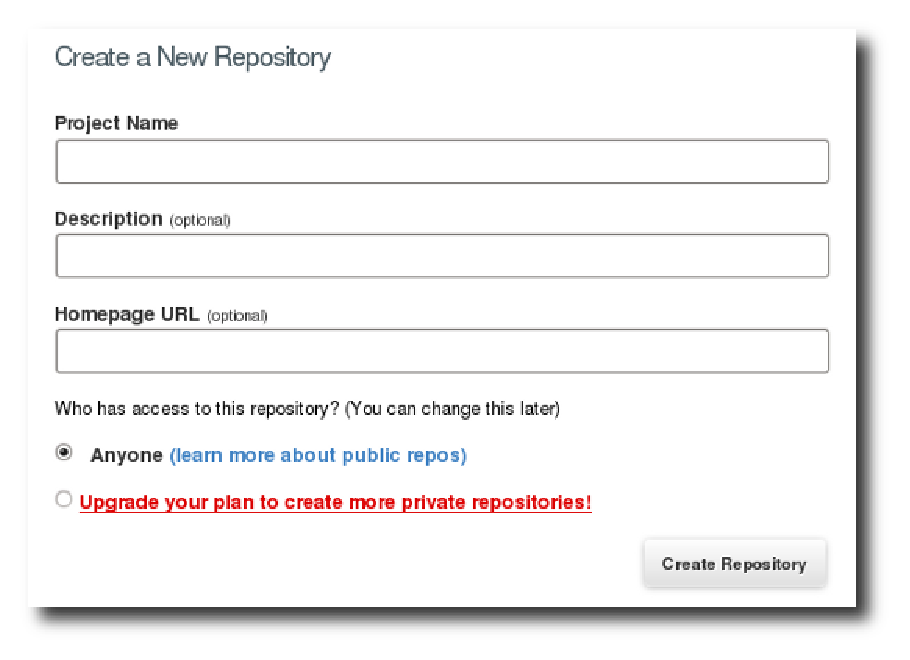
\includegraphics{Figures/GitHub_repo_details.eps}
  \end{center}
  \label{GitHub new repository details}
  \caption{GitHub new repository details}
\end{figure}

Once this done you can use the Git repository adress displayed on the top with
your favorite git client.

\begin{figure}[!htb]
  \begin{center}
    
\includegraphics{Figures/GitHub_repo_adress.eps}
  \end{center}
  \label{GitHub new repository adress}
  \caption{GitHub new repository adress}
\end{figure}


\paragraph{Create a README for your repo}
While a README isn’t a required part of a GitHub repo, it is a good idea to have
one. READMEs are a great place to describe your project or add some documentation
such as how to install or use your project.

If you include a file with the filename “README” in your repo, it will
automatically be shown on your repo’s front page. GitHub supports a number of
different README formats. Usually the README will result in a basic text
file but other formats like .markdown or .textile can be used to render HTML
content like links and headers.

\subsection{Why git?}
For a thorough discussion on the pros and cons of Git compared to centralized
source code control systems, see the web. As a developer, I prefer Git above all
other tools around today.

\subsubsection{cheap branching and easy merging}
Probably the most compelling feature of Git, since it often fundamentally changes
the way that many developers work, is Gits branching model. Instead of the
popular VCS branching method of simply cloning into a seperate directory for a
branch, Git lets you switch between branches in a single working directory. Add
to that the fact that creating and switching between branches is nearly instant,
not all of your branches need to be shared, and it’s easy to stash partially
completed work - means that the way you work can be incredibly different.

Instead of only having branches for major development line departures, Git
developers routinely create, merge and destroy multiple branches a week, or even
per day. Often each feature or bug you are working on can have its own branch,
merged in only when it is complete. This model allows you to experiment quickly,
easily and safely - without having to go through hoops to get back to where you
where. It enables and encourages a non-linear development cycle, where you can
work on multiple lines of thought in parallel without them stepping on each
other.

Many developers feel that this is so incredibly helpful and has changed their
workflow and productivity so much that they dub it the “killer feature” of Git.

\subsubsection{Offline and fast}
Git is fully distributed, which means that it can work almost entirely offline.
In stark contrast to VCS tools like Perforce or Subversion, Git does nearly all
of it’s operations without needing a network connection, including history
viewing, difference viewing and commiting.

This also means that Git is very fast compared to those systems partially due to
the fact that none of these operations has any dependency on network latency. For
example, take a look at how fast the simple ‘log’ command takes to run in Git and
in Subversion.

Git at 0.3 seconds vs Subversion at 3.7 seconds. That is a difference of a full
order of magnatude. You’ll find similar differences with nearly any command
comparison. For example, adding the popular famfamfam icon set and committing
them. Since you can seperate the commit from the network ‘push’ in Git, this
action takes a quarter of a second in Git, but 45 seconds in Subversion.

Even if you needed to push to a shared repository at that time as well, it still
takes far, far less time than Subversion.

If you just want to commit and keep working, you’re looking at a huge time
difference - one that severely changes your workflow. Most commands in Git seem
instantaneous - no more typing ‘svn commit’ and then going for a cup of coffee.

\begin{figure}
  \begin{center}
    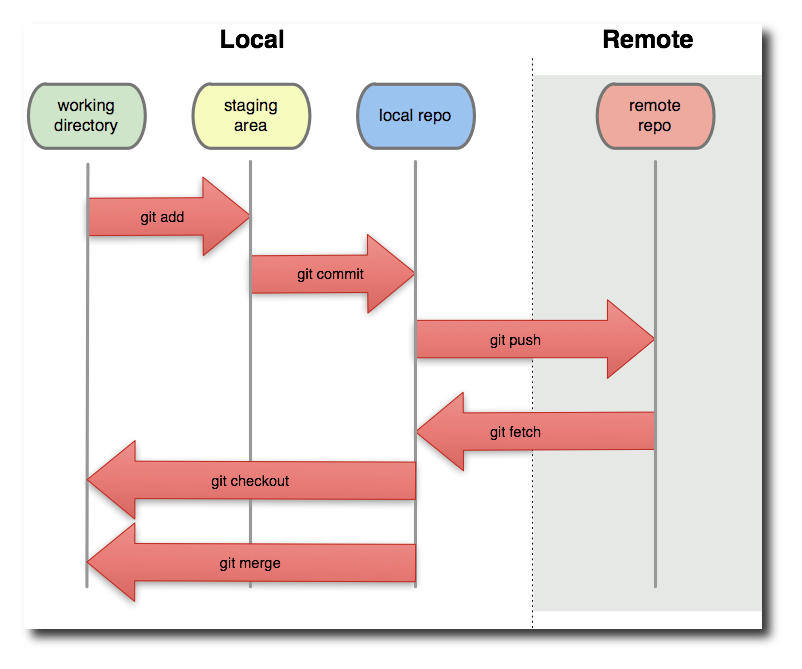
\includegraphics[scale=0.7]{Figures/Git_local.eps}
  \end{center}
  \caption{Git local-remote workflow}
  \label{Git local-remote workflow}
\end{figure}


\subsubsection{Small}
Git is also very space efficient. For example, if you import the Django project
from SVN into Git and compare their checkout/clone sizes, Git comes out very
favorably.
\begin{verbatim}
$ du -d 1 -h
 44M	./django-git
 53M	./django-svn
\end{verbatim}
Interestingly, it is even smaller than the Subversion checkout, which is pretty
amazing, considering that the Git clone contains the entire history of the
project - every version of every file back to the first commit, whereas the
Subversion checkout is just the last version of the project.


\subsubsection{Decentralized but centralized}
The repository setup that we use and that works well with this branching model,
is that with a central “truth” repo. Note that this repo is only considered to be
the central one (since Git is a DVCS, there is no such thing as a central repo at
a technical level).

Each developer pulls and pushes to origin. But besides the centralized push-pull
relationships, each developer may also pull changes from other peers to form sub
teams. For example, this might be useful to work together with two or more
developers on a big new feature, before pushing the work in progress to origin
prematurely.
